\section{Use Cases}

In diesem Kapitel werden die Anforderungen an die Software in Form von Use-Cases (Anwendungsfällen) dokumentiert. Die Use-Cases wurden aufgrund des Auftrages und weiteren Besprechungen mit dem Industriepartner definiert. Abbildung \ref{fig:usecases} zeigt eine Übersicht über die Use-Cases für den Agent sowie das Control Center.


\begin{figure}
  \centering
    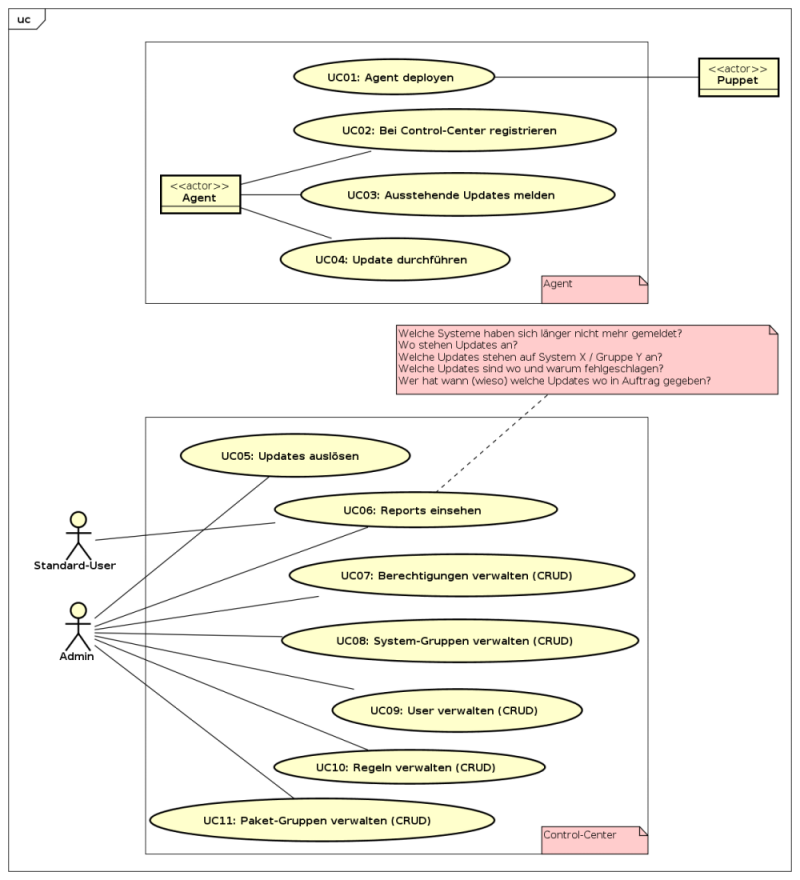
\includegraphics[width=0.9\textwidth]{files/UseCases_small}
  \caption{Übersicht der Use Cases}
  \label{fig:usecases}
\end{figure}

\subsection*{UC01: Agent deployen}
\label{sec:uc_01}

Der Agent wird auf einem System ausgeliefert. Dabei werden Parameter zur Konfiguration des Agents bei der Installation mitgegeben.


Technische Details:

\begin{itemize}
    \item Das Paket wird als .deb via Puppet ausgeliefert
    \item Konfiguration des Agents enthält: Adresse des Control-Centers und das CA-Zertifikat
\end{itemize}


\subsection*{UC02: Registration von Agent an Control Server}
\label{sec:uc_02}

Ein Agent registriert sich beim Control-Center.

Technische Details:

\begin{itemize}
    \item Registration geschieht über die beim Deployment erhaltene Adresse und dem generierten Zertifikat
    \item Der Agent übermittelt seinen Fully Qualified Domain Name
\end{itemize}

\subsection*{UC03: Ausstehende Updates melden}
\label{sec:uc_03}

Ein Agent aktualisiert die Paketliste. Er prüft, ob Updates anstehen und meldet diese Liste dem Control-Center. Gleichzeitig sendet er auch noch Hostinformationen, damit das Control-Center seine Informationen ggf. aktualisieren kann.
 

Technische Details:

\begin{itemize}
    \item Paketliste wird via apt-Schnittstelle aktualisiert
    \item Hostinformationen enthalten seine OS-Version sowie Hostnamen
\end{itemize}

\subsection*{UC04: Update durchführen}
\label{sec:uc_04}

Ein Agent erhält vom Control-Center einen Task mit einer Liste von vorzunehmenden System-Updates. Er prüft, ob diese bei sich anstehen und führt diese durch. Das Empfangen der Updates bestätigt er an das Control-Center, wo der Status dieses Tasks auf "Queued" gesetzt wird.

\subsection*{UC05: Update auslösen}
\label{sec:uc_05}

Das Control-Center hat eine Liste von ausstehenden Updates von einem oder mehreren Systemen erhalten. Diese zeigt es in einer Übersicht an. Ein User mit entsprechender Berechtigungs-Stufe gibt eines oder mehrere dieser Updates frei. Das Control-Center erstellt daraus Tasks, welche der User freigeben kann. Falls die Tasks freigegeben werden, schickt das Control-Center diese Tasks an die jeweiligen Systeme.

\subsection*{UC06: Statusreport anzeigen}
\label{sec:uc_06}

Ein User lässt sich vom Control-Center eine Liste von Systemen und Updates anzeigen. Darauf ersichtlich ist der Zustand jedes Systems und Updates. Der User sieht, auf welchem System ein Update aussteht und welche Updates in welchem Zustand sind.

\subsection*{UC07: Berechtigungen verwalten}
\label{sec:uc_07}

Ein Administrator kann für Systemgruppen und Paket-Gruppen Berechtigungs-Stufen setzen, so dass nur User mit dieser Stufe Aktionen auf diesen Gruppen vornehmen können.

\subsection*{UC08: System-Gruppen verwalten}
\label{sec:uc_08}

Ein Administrator kann eine System-Gruppe bearbeiten, löschen oder erstellen. Dies beinhaltet auch das Entfernen oder Hinzufügen von Systemen sowie das Setzen von Berechtigungs-Stufen.

\subsection*{UC09: User verwalten}
\label{sec:uc_09}

Ein Administrator kann neue User erstellen, bestehende User löschen oder deren Berechtigungs-Stufe ändern.

\subsection*{UC10: Regeln verwalten}
\label{sec:uc_10}

Ein Administrator kann Regeln für System-Gruppen erstellen, ändern und entfernen. Diese Regeln greifen bei der Auswahl der Systeme und Pakete.

\subsection*{UC11: Paket-Gruppen verwalten}
\label{sec:uc_11}

Ein Administrator kann neue Gruppen für Pakete erstellen, löschen oder bearbeiten. Dies beinhaltet auch das Entfernen oder Hinzufügen von Paketen sowie das Setzen von Berechtigungs-Stufen.
